% Copyright (c) 2022 by Lars Spreng
% This work is licensed under the Creative Commons Attribution 4.0 International License.

\documentclass[
11pt,notheorems,hyperref={pdfauthor=whatever}
]{beamer}

\usepackage{kotex}
\input{loadslides.tex}

\usepackage{fontspec}
\IfFontExistsTF{Pretendard}{%
  \setmainfont[
    UprightFont={Pretendard Medium},
    BoldFont={Pretendard Bold},
    ItalicFont={Pretendard Medium},
    BoldItalicFont={Pretendard Bold}
  ]{Pretendard}
  \setsansfont[
    UprightFont={Pretendard Medium},
    BoldFont={Pretendard Bold},
    ItalicFont={Pretendard Medium},
    BoldItalicFont={Pretendard Bold}
  ]{Pretendard}
  \setmonofont[
    UprightFont={Pretendard Medium},
    BoldFont={Pretendard Bold},
    ItalicFont={Pretendard Medium},
    BoldItalicFont={Pretendard Bold}
  ]{Pretendard}
  \setmainhangulfont[
    UprightFont={Pretendard Medium},
    BoldFont={Pretendard Bold},
    ItalicFont={Pretendard Medium},
    BoldItalicFont={Pretendard Bold}
  ]{Pretendard}
  \setsanshangulfont[
    UprightFont={Pretendard Medium},
    BoldFont={Pretendard Bold},
    ItalicFont={Pretendard Medium},
    BoldItalicFont={Pretendard Bold}
  ]{Pretendard}
  \setmonohangulfont[
    UprightFont={Pretendard Medium},
    BoldFont={Pretendard Bold},
    ItalicFont={Pretendard Medium},
    BoldItalicFont={Pretendard Bold}
  ]{Pretendard}
}{%
\IfFontExistsTF{NanumGothic}{%
  \setmainfont[
    UprightFont=NanumGothicBold,
    BoldFont=NanumGothicBold
  ]{NanumGothic}
  \setsansfont[
    UprightFont=NanumGothicBold,
    BoldFont=NanumGothicBold
  ]{NanumGothic}
  \setmonofont[
    UprightFont=NanumGothicBold,
    BoldFont=NanumGothicBold
  ]{NanumGothic}
  \setmainhangulfont[
    UprightFont=NanumGothicBold,
    BoldFont=NanumGothicBold
  ]{NanumGothic}
  \setsanshangulfont[
    UprightFont=NanumGothicBold,
    BoldFont=NanumGothicBold
  ]{NanumGothic}
  \setmonohangulfont[
    UprightFont=NanumGothicBold,
    BoldFont=NanumGothicBold
  ]{NanumGothic}
}{%
  \IfFontExistsTF{Nanum Gothic}{%
    \setmainfont[
      UprightFont=Nanum Gothic Bold,
      BoldFont=Nanum Gothic Bold
    ]{Nanum Gothic}
    \setsansfont[
      UprightFont=Nanum Gothic Bold,
      BoldFont=Nanum Gothic Bold
    ]{Nanum Gothic}
    \setmonofont[
      UprightFont=Nanum Gothic Bold,
      BoldFont=Nanum Gothic Bold
    ]{Nanum Gothic}
    \setmainhangulfont[
      UprightFont=Nanum Gothic Bold,
      BoldFont=Nanum Gothic Bold
    ]{Nanum Gothic}
    \setsanshangulfont[
      UprightFont=Nanum Gothic Bold,
      BoldFont=Nanum Gothic Bold
    ]{Nanum Gothic}
    \setmonohangulfont[
      UprightFont=Nanum Gothic Bold,
      BoldFont=Nanum Gothic Bold
  ]{Nanum Gothic}
  }{}%
}}
\renewcommand{\familydefault}{\sfdefault}

\usepackage{tikz}
\usetikzlibrary{arrows.meta, positioning, calc, fit, backgrounds, shapes.geometric}
\usepackage{booktabs}
\usepackage{array}
\usepackage{tabularx}
\usepackage{adjustbox}

\definecolor{TextGray}{HTML}{333333}
\definecolor{DeepBlue}{HTML}{08457E}
\definecolor{SoftBlue}{HTML}{EAF0F8}
\definecolor{LineGray}{HTML}{B8B8B8}
\definecolor{WarnRed}{HTML}{B3261E}
\definecolor{GoodGreen}{HTML}{237A4B}
\definecolor{SoftGreen}{HTML}{EAF6EF}
\definecolor{SoftRed}{HTML}{FBEAEA}
\definecolor{SoftYellow}{HTML}{FFF4D8}
\definecolor{SoftPurple}{HTML}{F1EAFE}

\addtobeamertemplate{frametitle}{}{\vspace{-0.5em}}
\setbeamerfont{title}{size=\LARGE,series=\bfseries}
\setbeamerfont{subtitle}{size=\large}
\setbeamerfont{frametitle}{series=\bfseries}

\tikzset{
  box/.style={draw=DeepBlue, very thick, rounded corners=2pt, fill=SoftBlue, align=center, minimum height=0.75cm, inner sep=5pt, font=\small\bfseries},
  smallbox/.style={draw=LineGray, rounded corners=2pt, fill=white, align=center, minimum height=0.55cm, inner sep=4pt, font=\scriptsize},
  greenbox/.style={draw=GoodGreen, very thick, rounded corners=2pt, fill=SoftGreen, align=center, minimum height=0.75cm, inner sep=5pt, font=\small\bfseries},
  redbox/.style={draw=WarnRed, very thick, rounded corners=2pt, fill=SoftRed, align=center, minimum height=0.75cm, inner sep=5pt, font=\small\bfseries},
  yellowbox/.style={draw=orange!70!black, very thick, rounded corners=2pt, fill=SoftYellow, align=center, minimum height=0.75cm, inner sep=5pt, font=\small\bfseries},
  purplebox/.style={draw=purple!70!black, very thick, rounded corners=2pt, fill=SoftPurple, align=center, minimum height=0.75cm, inner sep=5pt, font=\small\bfseries},
  arrow/.style={-{Latex[length=2.5mm]}, thick, draw=DeepBlue},
  grayarrow/.style={-{Latex[length=2.2mm]}, thick, draw=LineGray},
  redarrow/.style={-{Latex[length=2.2mm]}, thick, draw=WarnRed},
  greenarrow/.style={-{Latex[length=2.2mm]}, thick, draw=GoodGreen}
}

\newcommand{\term}[1]{\textbf{\textcolor{DeepBlue}{#1}}}
\newcommand{\smallgray}[1]{{\scriptsize\textcolor{gray!75}{#1}}}

\title[]{7/14 미팅}
\subtitle{Dual-Channel Latent Communication for Clinical Diagnosis}
\author[]{하서준}
\institute{DGIST}
\date{2026년 7월 14일}

\begin{document}

{
\setbeamertemplate{footline}{}
\begin{frame}
  \titlepage
  \vspace{-0.8em}
  \begin{center}
  \scriptsize
  C2C \(\cdot\) LCF \(\cdot\) LR Agent \(\cdot\) LoRA Cache Handoff
  \end{center}
\end{frame}
}
\addtocounter{framenumber}{-1}

\begin{frame}[t]{기존 latent communication은 대체로 하나의 매체를 선택한다}
\scriptsize
\begin{center}
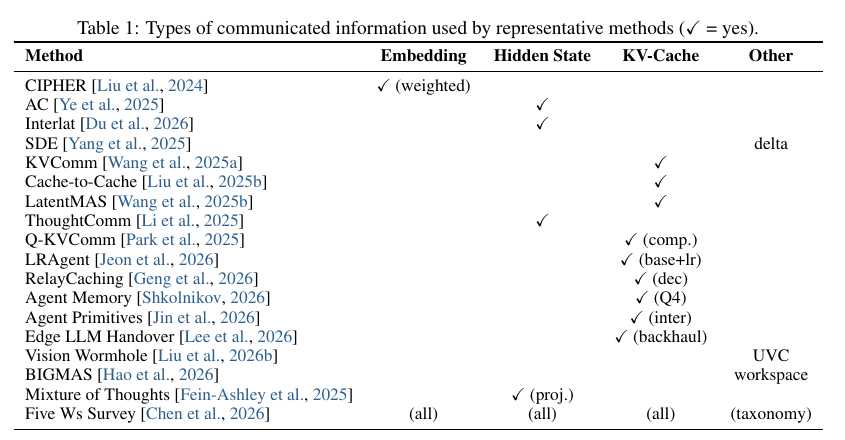
\includegraphics[width=1.02\linewidth,height=0.66\textheight,keepaspectratio]{figures/lantet_종류.png}
\end{center}

\vfill
\begin{center}
\normalsize
\fcolorbox{DeepBlue}{SoftBlue}{\parbox{0.92\linewidth}{
\centering
기존 latent communication 연구들은 모두 embedding, hidden state, KV-cache 중\\
\term{하나의 latent 매체}만 선택해 넘겨왔다.\\
\vspace{0.25em}
\textbf{그러나 이들이 정말 같은 정보인가?}
}}
\end{center}
\end{frame}

\begin{frame}[t]{Latent communication에서 넘길 수 있는 신호 종류}
\scriptsize
\begin{columns}[T,onlytextwidth]
\begin{column}{0.47\textwidth}
\begin{center}
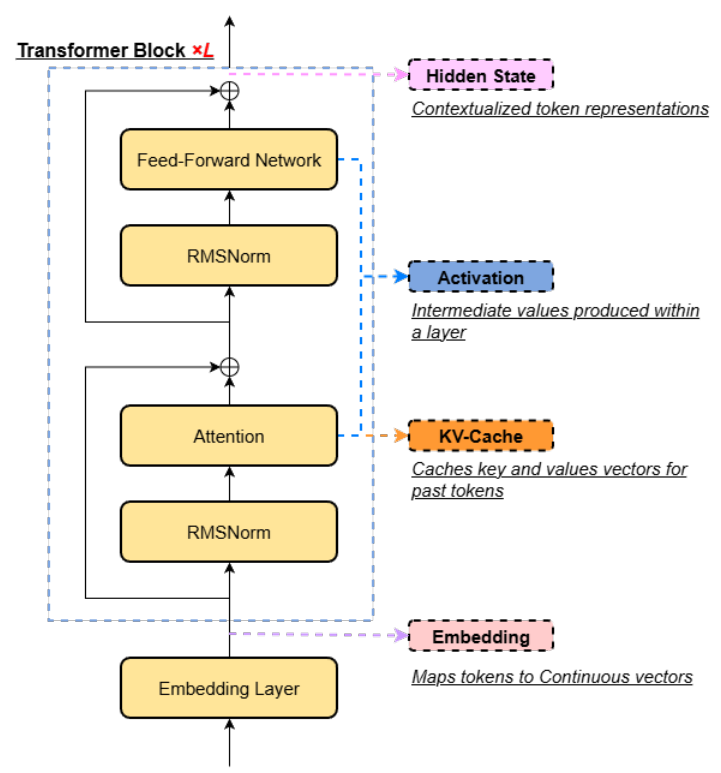
\includegraphics[width=1.06\linewidth,height=0.82\textheight,keepaspectratio]{figures/latent종류.png}
\end{center}
\end{column}
\begin{column}{0.50\textwidth}
\textbf{어떤 latent를 넘기는지에 따라 의미가 달라진다}
\vspace{0.9em}

\begin{itemize}
\setlength{\itemsep}{1.35em}
  \item \textbf{Hidden state}\\
  현재 prefix를 처리한 compact representation. belief나 intent를 압축해 전달하기 좋지만, token-level evidence memory는 약하다.

  \item \textbf{KV cache}\\
  attention에서 다시 참조할 수 있는 context memory. long evidence를 보존하지만, base memory와 role-specific signal이 섞인다.

  \item \textbf{Embedding}\\
  token이 transformer block에 들어가기 전의 lexical input representation. 원문 token identity는 강하지만,
  reasoning 이후의 belief나 attention memory는 아직 담기지 않는다.
\end{itemize}

\vspace{1.25em}
\fcolorbox{GoodGreen}{SoftGreen}{\parbox{0.92\linewidth}{
\textbf{핵심:} embedding은 입력 자체, hidden state는 compact belief, KV cache는 다시 참조 가능한 evidence memory에 가깝다.
}}
\end{column}
\end{columns}
\end{frame}

\begin{frame}[t]{왜 KV와 hidden state를 둘 다 넘기는가?}
\small
\vspace{0.7em}
\begin{columns}[T,onlytextwidth]
\begin{column}{0.46\textwidth}
\centering
\textbf{\Large KV cache}
\vspace{0.8em}

\raggedright
\begin{itemize}
  \setlength{\itemsep}{0.9em}
  \item prompt와 patient evidence를 token-level로 다시 참조할 수 있는 cache
  \item 모델의 생각이 발전하면서 어떤 evidence를 누적했는지 보존
  \item attention 과정에서 어떤 부분에 집중했는지 반영
  \item planner가 필요한 증거 위치에 다시 cross-attend할 수 있음
\end{itemize}

\vspace{0.7em}
\textbf{역할}\\
``무엇을 봤는가''를 담는\\
diagnostic evidence memory
\end{column}

\begin{column}{0.04\textwidth}
\centering
\rule{0.7pt}{0.68\textheight}
\end{column}

\begin{column}{0.46\textwidth}
\centering
\textbf{\Large Hidden state}
\vspace{0.8em}

\raggedright
\begin{itemize}
  \setlength{\itemsep}{0.9em}
  \item decode 직전 next-token prediction으로 이어지는 집약 representation
  \item 마지막 hidden state는 LM head를 거쳐 logits로 바로 변환
  \item disease posterior와 uncertainty를 compact하게 표현
  \item stop/add gate와 action policy에 직접 연결하기 쉬움
\end{itemize}

\vspace{0.7em}
\textbf{역할}\\
``현재 무엇을 믿는가''를 담는\\
diagnostic belief state
\end{column}
\end{columns}
\end{frame}

\begin{frame}[t]{구조: Dual Channel Latent Communication}
\scriptsize
\begin{center}
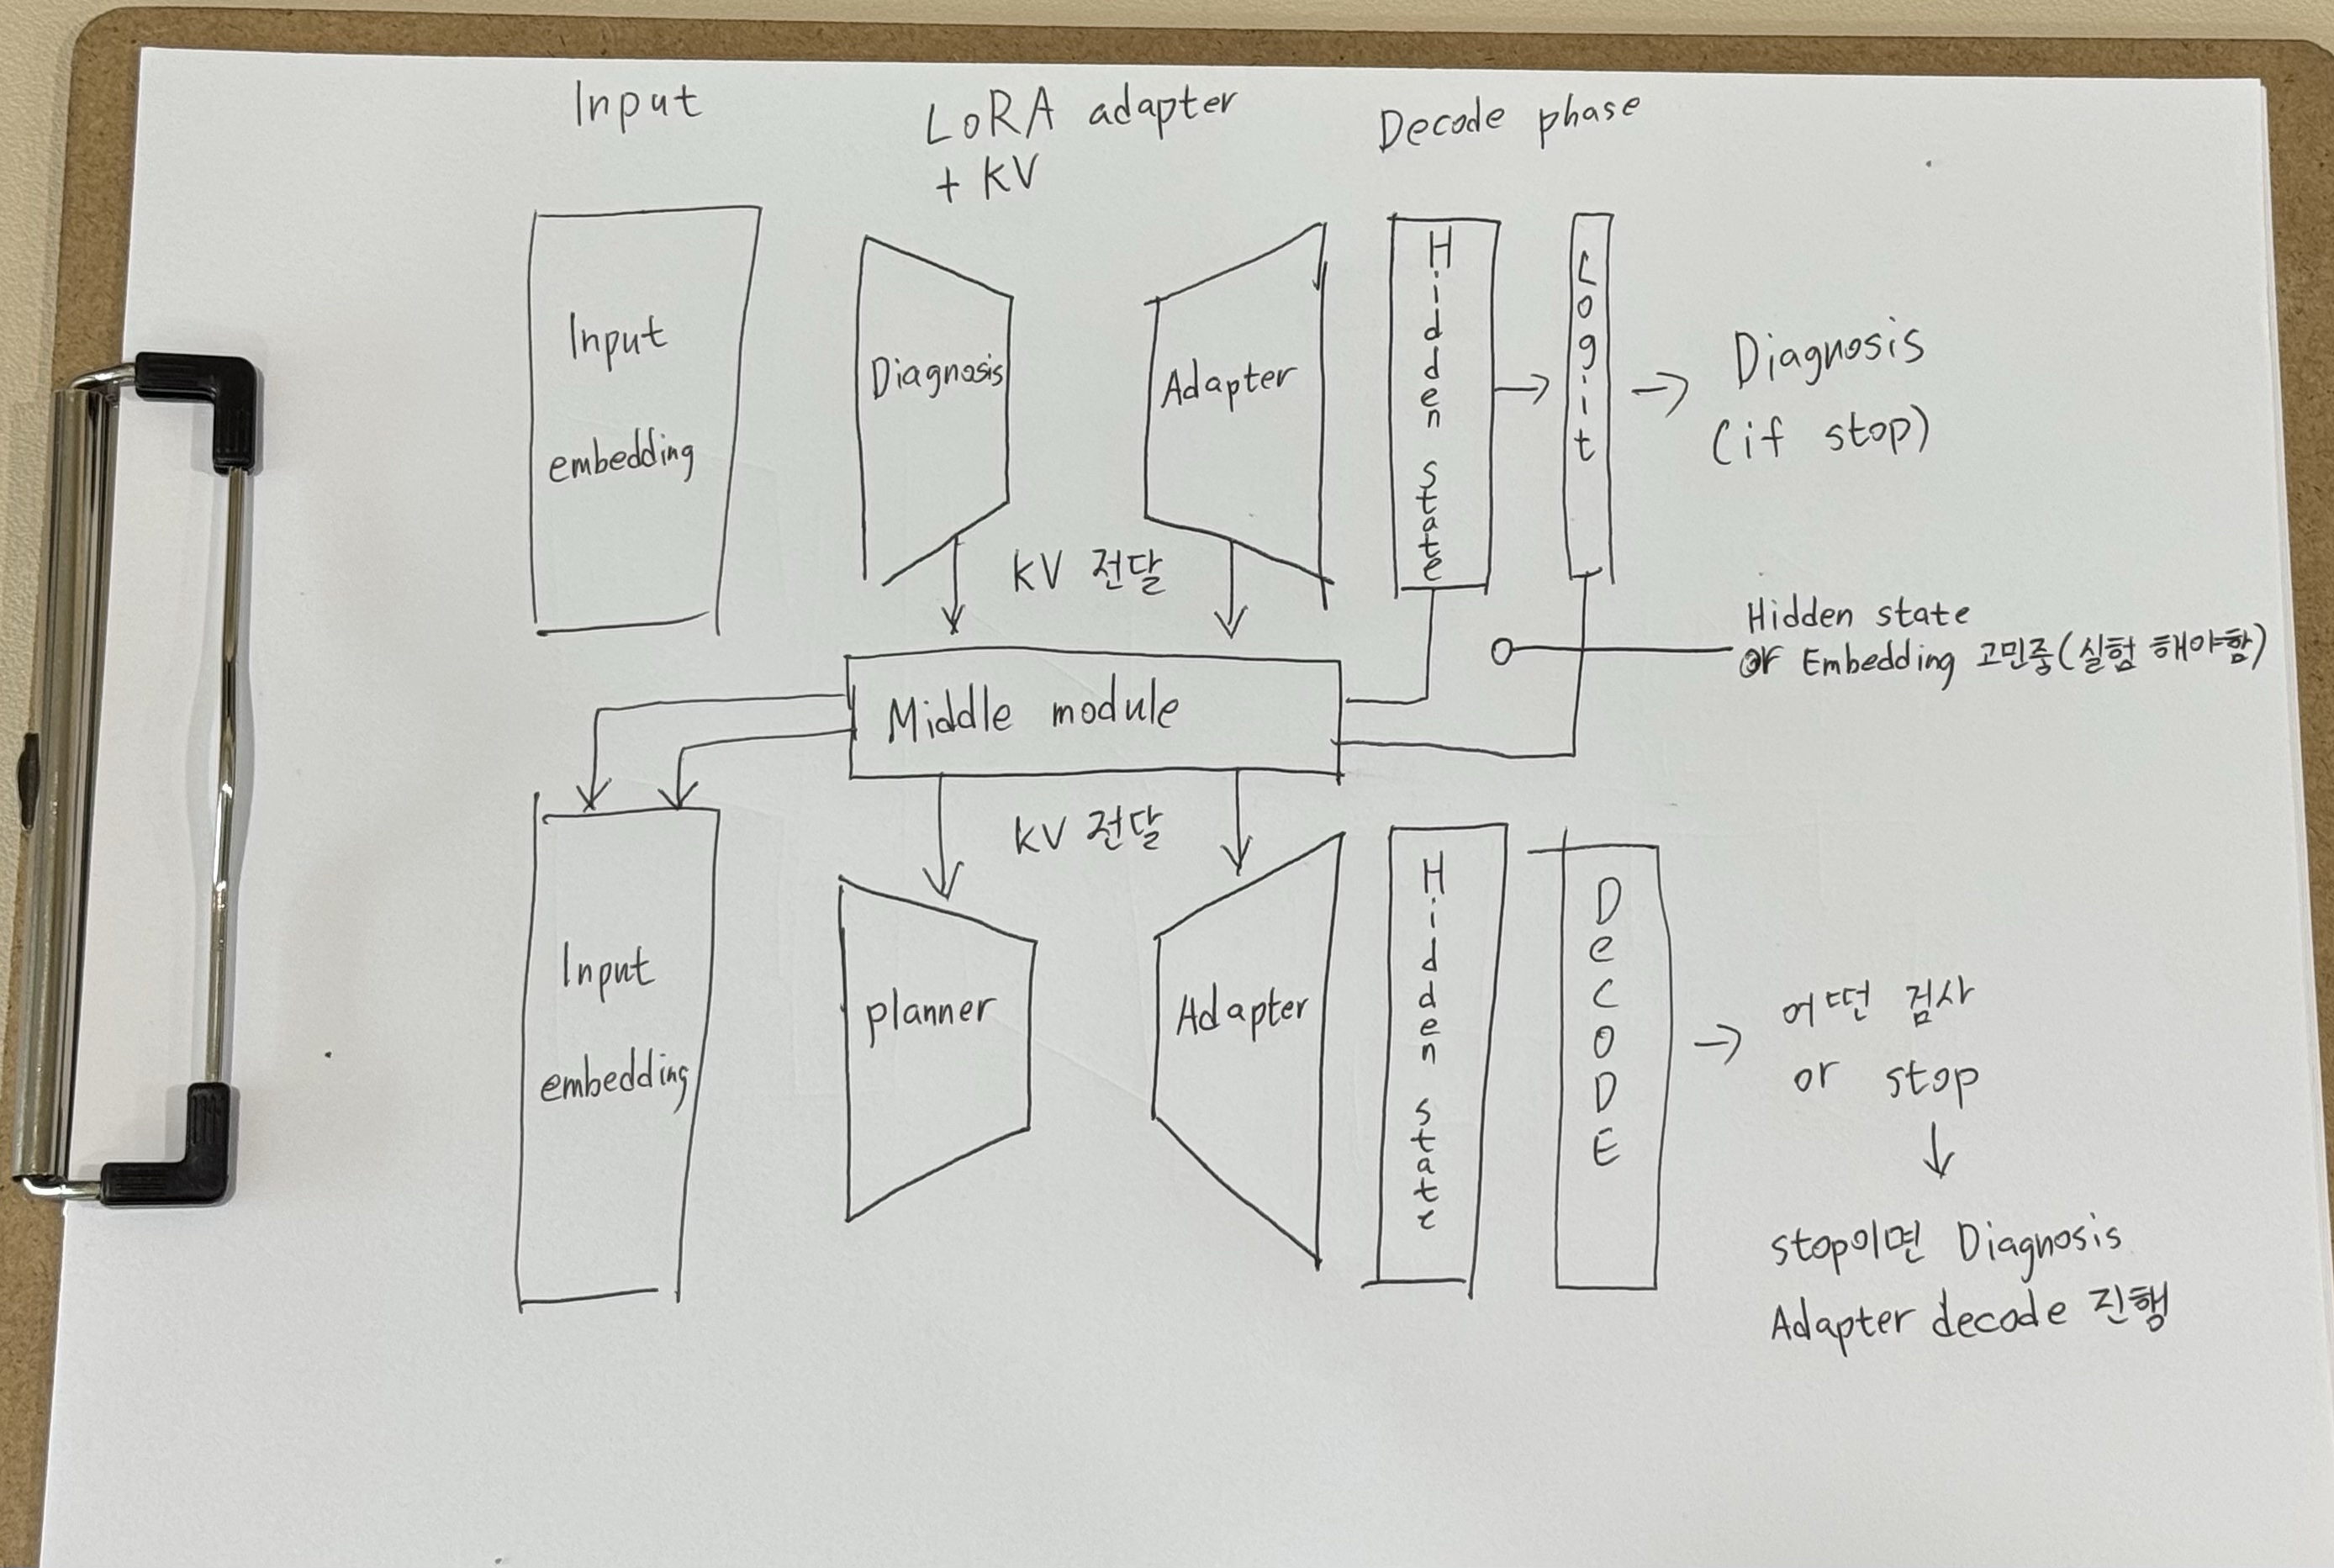
\includegraphics[width=1.06\linewidth,height=0.84\textheight,keepaspectratio]{figures/image.jpeg}
\end{center}

\end{frame}

\begin{frame}[t]{LR Agent: 멀티 LoRA adapter 세팅에서 캐시를 공유해보자}
\scriptsize
\textbf{multi-LoRA weight decomposition}
\vspace{0.15em}

\begingroup
\Large
\[
W_i = W_0 + \Delta W_i = W_0 + A_iB_i
\]
\[
Y_i = X_iW_i
    = X_iW_0 + (X_iA_i)B_i
\]
\endgroup

\vspace{0.15em}
\begin{center}
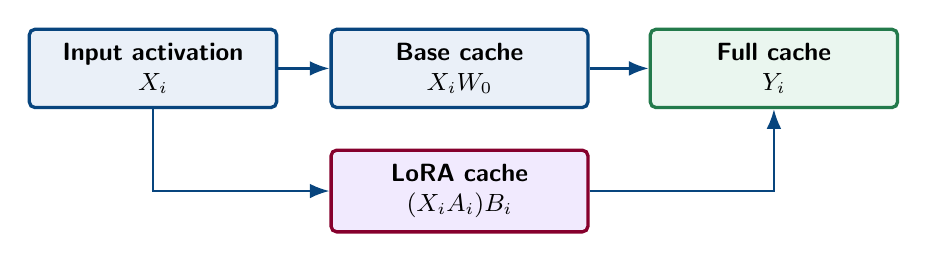
\begin{tikzpicture}[node distance=0.7cm]
\node[box, text width=0.23\linewidth] (x) {
\textbf{Input activation}\\
\(X_i\)
};
\node[box, right=0.65cm of x, text width=0.24\linewidth] (base) {
\textbf{Base cache}\\
\(X_iW_0\)
};
\node[purplebox, below=0.5cm of base, text width=0.24\linewidth] (lora) {
\textbf{LoRA cache}\\
\((X_iA_i)B_i\)
};
\node[greenbox, right=0.75cm of base, text width=0.23\linewidth] (sum) {
\textbf{Full cache}\\
\(Y_i\)
};
\draw[arrow] (x) -- (base);
\draw[arrow] (x) |- (lora);
\draw[arrow] (base) -- (sum);
\draw[arrow] (lora) -| (sum);
\end{tikzpicture}
\end{center}

\vspace{0.3em}
\textbf{KV cache에 적용하면}
\[
V_i = V_{\text{base},i} + V_{\text{adapter},i},
\quad
V_{\text{adapter},i} = (X_iA_i^V)B_i^V
\]

\begin{itemize}
  \item LR Agent는 base cache를 agent 간 공유하고, adapter output은 low-rank cache로 저장한다.
  \item 여기서 중요한 건 \term{full KV가 아니라 adapter-induced cache residual을 따로 볼 수 있다}는 점이다.
\end{itemize}
\end{frame}

\begin{frame}[t]{KV 넘기는 구조}
\scriptsize
\begin{center}
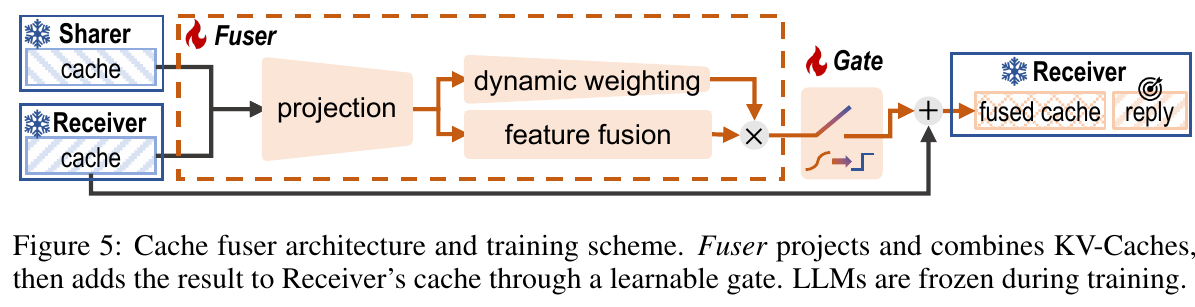
\includegraphics[width=0.94\linewidth,height=0.28\textheight,keepaspectratio]{figures/C2C.png}
\end{center}

\vspace{0.25em}
\begin{columns}[T,onlytextwidth]
\begin{column}{0.92\textwidth}
\textbf{핵심 아이디어}
\begin{itemize}
  \item Sender가 만든 \(KV_s\)를 receiver가 쓸 수 있는 \(\hat{KV}_r\)로 변환한다.
  \item 자연어 메시지 대신 latent cache를 직접 넘기므로 정보 손실과 재-prefill 비용을 줄일 수 있다.
  \item 하지만 보통 full KV를 대상으로 하므로 base memory와 role-specific adaptation이 분리되지 않는다.
\end{itemize}

\vspace{0.2em}
\textbf{우리 관점에서의 한계}
\begin{itemize}
  \item planner가 필요한 것은 전체 source context가 아니라 diagnosis adapter가 만든 diagnostic delta다.
  \item 따라서 full KV handoff보다 LoRA-induced cache만 fusion하는 편이 더 직접적이다.
\end{itemize}
\end{column}
\end{columns}
\end{frame}

\end{document}

\begin{frame}[t]{왜 latent communication이 필요한가?}
\scriptsize
\textbf{기존 LLM-based MAS의 기본 구조}
\vspace{0.35em}

\begin{center}

\includegraphics[
  width=1.04\linewidth,
  height=0.43\textheight,
  keepaspectratio
]{figures/why_latent.png}
\end{center}

\vspace{0.75em}
\textbf{\textcolor{WarnRed}{Text-only communication의 세 가지 한계}}
\vspace{0.2em}
\begin{enumerate}
  \item \textbf{높은 inference cost}\\
  모든 메시지마다 sender는 token을 생성하고, receiver는 그 token을 다시 encoding해야 한다.

  \item \textbf{Discretization 과정의 정보 손실}\\
  고차원 hidden state가 vocabulary token 하나로 압축된다.
  논문은 token의 정보량을 대략 \(15\)--\(17\) bits로 보고, hidden state는 훨씬 큰 capacity를 가진다고 설명한다.

  \item \textbf{자연어의 중복성과 모호성}\\
  자연어는 사람이 읽기 좋지만 장황하고, hedge 표현이나 모호한 지시어 때문에 task-relevant density가 낮을 수 있다.
\end{enumerate}
\end{frame}

\begin{frame}[t]{Prefill phase와 Decode phase}
\small
\textbf{LLM inference는 크게 두 단계로 나뉜다.}

\vspace{0.2em}
\begin{center}

\includegraphics[
  width=0.74\linewidth,
  height=0.30\textheight,
  keepaspectratio
]{figures/prefill_decode.png}
\end{center}

\vspace{0.15em}
\begin{columns}[T,onlytextwidth]
\begin{column}{0.49\textwidth}
\textbf{\textcolor{DeepBlue}{Prefill phase}}
\begin{itemize}
  \item 입력 prompt 전체를 한 번에 Transformer에 통과시킨다.
  \item 모든 input token의 hidden state와 KV-cache가 만들어진다.
  \item prompt가 길수록 비용이 크게 증가한다.
\end{itemize}
\end{column}

\begin{column}{0.49\textwidth}
\textbf{\textcolor{DeepBlue}{Decode phase}}
\begin{itemize}
  \item 만들어진 KV-cache를 사용해 다음 token을 하나씩 생성한다.
  \item 각 step에서는 직전 token과 누적 KV-cache를 참조한다.
  \item 생성 길이에 비례해 반복적으로 비용이 든다.
\end{itemize}
\end{column}
\end{columns}

\vspace{0.35em}
\begin{center}
\fcolorbox{WarnRed}{SoftRed}{\parbox{0.86\linewidth}{\centering
Prefill에서는 모든 input token의 hidden state와 KV-cache가 생성되고,
decode에서는 최신 token의 hidden state와 계속 커지는 KV-cache가 핵심 latent가 된다.
}}
\end{center}
\end{frame}

\begin{frame}[t]{무엇이 달라질 수 있나?}
\small
\textbf{핵심 아이디어:} agent가 자연어를 생성하지 않고 내부 연속 표현을 직접 전달한다.

\vspace{0.45em}
\begin{center}
\begin{tikzpicture}[node distance=0.75cm]
\node[box, minimum width=2.5cm] (sender) {보내는 agent};
\node[greenbox, right=0.8cm of sender, minimum width=3.0cm] (latent) {Embedding\\Hidden State\\KV-Cache};
\node[box, right=0.8cm of latent, minimum width=2.5cm] (receiver) {받는 agent};
\draw[arrow] (sender) -- (latent);
\draw[arrow] (latent) -- (receiver);
\node[redbox, below=0.7cm of latent, minimum width=5.6cm] (skip) {vocabulary bottleneck 우회};
\draw[redarrow] (skip) -- (latent);
\end{tikzpicture}
\end{center}

\vspace{0.4em}
\textbf{이 논문의 3-axis 분석 틀}
\vspace{0.2em}
\begin{columns}[T,onlytextwidth]
\begin{column}{0.32\textwidth}
\fcolorbox{DeepBlue}{SoftBlue}{\parbox{0.9\linewidth}{\centering
\textbf{WHAT}\\
무엇을 보낼까?\\
\scriptsize Embedding / Hidden State / KV-Cache
}}
\end{column}
\begin{column}{0.32\textwidth}
\fcolorbox{DeepBlue}{SoftBlue}{\parbox{0.9\linewidth}{\centering
\textbf{WHICH}\\
어디에 맞출까?\\
\scriptsize layer / latent alignment
}}
\end{column}
\begin{column}{0.32\textwidth}
\fcolorbox{DeepBlue}{SoftBlue}{\parbox{0.9\linewidth}{\centering
\textbf{HOW}\\
어떻게 합칠까?\\
\scriptsize concatenate / prepend / fuse
}}
\end{column}
\end{columns}

\vspace{0.45em}
\begin{center}
\fcolorbox{LineGray}{white}{\parbox{0.82\linewidth}{\centering
\[
\text{방법}
=(
\underbrace{\text{WHAT}}_{\text{정보 종류}},
\underbrace{\text{WHICH}}_{\text{alignment}},
\underbrace{\text{HOW}}_{\text{fusion}}
)
\]
}}
\end{center}
\end{frame}

\begin{frame}[t]{자연어 vs. Latent communication: 언제 무엇을 쓰나?}
\footnotesize
\textbf{Latent communication이 natural language를 완전히 대체하는 것은 아니다.}
\vspace{1.25em}

\begin{columns}[T,onlytextwidth]
\begin{column}{0.49\textwidth}
\fcolorbox{DeepBlue}{SoftBlue}{\parbox{0.93\linewidth}{
\centering\textbf{자연어 Communication}
\vspace{0.15em}
}}

\vspace{0.3em}
\textbf{자연어를 사용해야 하는 경우}
\begin{itemize}
  \item \textbf{사람의 해석이 필요할 때}
  \item 자연어 message는 사람이 즉시 읽을 수 있음
  \item debugging, alignment auditing, safety review에 유리
  \item human--AI interaction에서 그대로 설명하고 검토 가능
\end{itemize}

\textbf{사용할 때}
\begin{itemize}
  \item final answer를 제공할 때
  \item 사용자에게 justification을 보여줘야 할 때
  \item human oversight / cross-organization interoperability 필요
\end{itemize}

\end{column}

\begin{column}{0.49\textwidth}
\fcolorbox{GoodGreen}{SoftGreen}{\parbox{0.93\linewidth}{
\centering\textbf{Latent Communication}
\vspace{0.15em}
}}

\vspace{0.3em}
\textbf{Latent를 선호하는 경우}
\begin{itemize}
  \item \textbf{강하게 연결된 agents}\\
  planner \(\rightarrow\) executor처럼 바로 이어지는 agents
  \item \textbf{중간 communication}\\
  사용자가 message를 볼 필요가 없는 단계
  \item \textbf{공유되거나 정렬된 latent space}\\
  same backbone 또는 compatible architectures
  \item \textbf{latency가 핵심 제약인 경우}\\
  real-time pipeline, edge deployment, large agent counts
\end{itemize}

\end{column}
\end{columns}

\end{frame}

\begin{frame}[t]{WHICH: 송신자와 수신자를 어디서 맞출까?}
\small
\vspace{0.7em}
\begin{enumerate}
  \item \textbf{\textcolor{DeepBlue}{Space: latent space를 맞춤}}\\
  \normalsize 같은 model은 거의 바로 공유 가능하다.
  같은 backbone의 fine-tune은 projection head로 맞출 수 있고,
  heterogeneous model은 learned alignment가 필요하다.

  \vspace{0.85em}
  \item \textbf{\textcolor{DeepBlue}{Layer: 어느 layer를 연결할지 정함}}\\
  \normalsize 대표적으로
  \textbf{Last \(\rightarrow\) First},
  \textbf{All \(\rightarrow\) Corresponding},
  \textbf{Selected \(\rightarrow\) Selected}가 있다.

  \vspace{0.85em}
  \item \textbf{\textcolor{DeepBlue}{Select: 필요한 일부만 고름}}\\
  \normalsize 모든 layer를 넘기면 정보는 많지만 비용이 크다.
  task와 receiver에 중요한 layer만 고르면 latency와 memory를 줄일 수 있다.
\end{enumerate}

\vspace{0.75em}
\begin{center}
\fcolorbox{DeepBlue}{SoftBlue}{\parbox{0.86\linewidth}{\centering
즉 WHICH는 \textbf{공간 정렬(Space)}, \textbf{레이어 매핑(Layer)},
\textbf{선택적 전달(Select)}의 문제로 볼 수 있다.
}}
\end{center}
\end{frame}

\begin{frame}[t]{HOW: 수신자의 computation에 어떻게 합칠까?}
\small
\vspace{0.8em}
\begin{enumerate}
  \item \textbf{\textcolor{DeepBlue}{Concat: latent token을 뒤에 붙임}}\\
  \normalsize Embedding/hidden state를 receiver sequence axis에 추가한다.
  가장 단순하지만 sequence length가 늘어난다.

  \vspace{0.85em}
  \item \textbf{\textcolor{DeepBlue}{Prepend: KV-cache 앞에 붙임}}\\
  \normalsize Sender KV를 receiver cache 앞에 두어 과거 memory처럼 attention하게 한다.
  KV-cache 계열의 기본 방식이다.

  \vspace{0.85em}
  \item \textbf{\textcolor{DeepBlue}{Fuse: projection 후 섞음}}\\
  \normalsize Add, gate, cross-attention 등으로 sender latent를 receiver computation에 섞는다.
  가장 유연하지만 alignment와 training이 필요하다.
\end{enumerate}

\vspace{0.8em}
\begin{center}
\fcolorbox{DeepBlue}{SoftBlue}{\parbox{0.86\linewidth}{\centering
직관적으로는 \textbf{붙이기(Concat)}, \textbf{기억으로 앞에 두기(Prepend)},
\textbf{계산해서 섞기(Fuse)}의 세 가지로 볼 수 있다.
}}
\end{center}
\end{frame}

\begin{frame}[t]{실험적 관찰: 무엇이 잘 먹히나?}
\vspace{2.4em}
\Large
\begin{center}
\begin{minipage}{0.86\linewidth}
\begin{enumerate}
  \item \textbf{\textcolor{DeepBlue}{Long context일수록 이득이 큼}}\\
  \normalsize receiver가 긴 prompt를 다시 encoding하지 않아도 되기 때문.

  \vspace{1.0em}
  \Large
  \item \textbf{\textcolor{DeepBlue}{Same-model agents가 지배적}}\\
  \normalsize 대부분 sender와 receiver가 같은 backbone을 공유한다고 가정.

  \vspace{1.0em}
  \Large
  \item \textbf{\textcolor{DeepBlue}{KV-cache가 emerging default}}\\
  \normalsize 18개 방법 중 9개가 KV-cache를 communicated quantity로 사용.
\end{enumerate}

\vspace{1.0em}
\large
\textbf{\textcolor{WarnRed}{핵심 trade-off}}:
정보량이 많을수록 latency는 줄기 쉽지만,
payload와 architecture dependence는 커진다.
\end{minipage}
\end{center}
\end{frame}

\begin{frame}[t]
\vspace{-0.35em}
{\large\bfseries Latent Collaboration in Multi-Agent Systems}\\[-0.1em]
{\scriptsize ICML, 2026}

\vspace{0.35em}
\begin{center}

\includegraphics[
  width=0.92\textwidth,
  height=0.70\textheight,
  keepaspectratio
]{figures/LatentMAS.png}
\end{center}

\vspace{0.1em}
\begin{center}
\fcolorbox{DeepBlue}{SoftBlue}{\parbox{0.91\linewidth}{\centering\small
자연어 communication은 느리고 hidden reasoning을 버린다.
\\ \textbf{\(\Rightarrow\) latent thought와 KV-cache를 다음 agent의 memory로 직접 넘기자.}
}}
\end{center}
\end{frame}

\begin{frame}[t]
\vspace{-0.35em}
{\large\bfseries Recursive Multi-Agent Systems}\\[-0.1em]
{\scriptsize arXiv, 2026}

\vspace{0.35em}
\begin{center}

\includegraphics[
  width=0.92\textwidth,
  height=0.69\textheight,
  keepaspectratio
]{figures/RecursiveMAS.png}
\end{center}

\vspace{0.1em}
\begin{center}
\fcolorbox{DeepBlue}{SoftBlue}{\parbox{0.91\linewidth}{\centering\small
MAS를 text message들의 왕복으로 보면 느리고 학습이 끊긴다.
\\ \textbf{\(\Rightarrow\) agent들을 latent recursion loop로 묶고 RecursiveLink만 학습하자.}
}}
\end{center}
\end{frame}

\begin{frame}[t]
\vspace{-0.35em}
{\large\bfseries Cache-to-Cache: Direct Semantic Communication}\\[-0.1em]
{\large\bfseries Between Large Language Models}\\[-0.1em]
{\scriptsize ICLR, 2026}

\vspace{0.15em}
\begin{center}
\makebox[\textwidth][c]{%
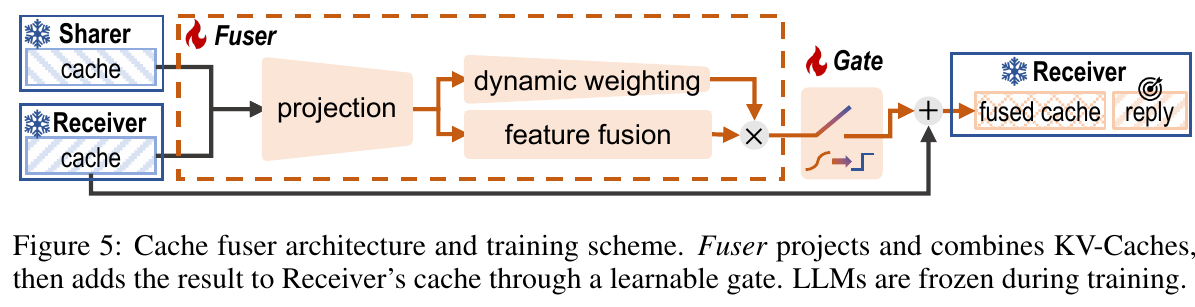
\includegraphics[
  width=0.96\paperwidth,
  keepaspectratio
]{figures/C2C.png}%
}
\end{center}

\vspace{0.25em}
\begin{center}
\fcolorbox{DeepBlue}{SoftBlue}{\parbox{0.91\linewidth}{\centering\small
기존 전달 방식은 sharer 정보에 집중하고 receiver의 현재 맥락은 충분히 보지 않는다.
\\ \textbf{\(\Rightarrow\) sharer/receiver KV를 함께 보고, 필요한 비율만 receiver cache에 주입하자.}
}}
\end{center}
\end{frame}

\begin{frame}[t]{Related works: 핵심 아이디어}
\small
\vspace{0.05em}
\renewcommand{\arraystretch}{1.7}
\begin{tabularx}{\linewidth}{@{}>{\raggedright\arraybackslash}p{0.18\linewidth}>{\raggedright\arraybackslash}X@{}}
\toprule
\textbf{논문/계열} & \textbf{기존 문제와 제안} \\
\midrule
\parbox[t]{0.18\linewidth}{\footnotesize\textbf{LRAgent}\\[-0.05em]{\tiny ICML'26}} &
\parbox[t]{0.88\linewidth}{Multi-LoRA agent는 backbone은 공유해도 같은 trajectory의 KV-cache를 agent별로 따로 만든다.\\[-0.05em]
\textbf{\(\Rightarrow\) base KV는 공유하고 LoRA 차이는 low-rank cache로만 저장하자.}} \\[0.5em]

\parbox[t]{0.18\linewidth}{\footnotesize\textbf{KVComm}\\[-0.05em]{\tiny NeurIPS'25}} &
\parbox[t]{0.88\linewidth}{Multi-agent workflow에서 같은 context가 반복되지만 agent별 prefix 때문에 KV-cache offset이 달라진다.\\[-0.05em]
\textbf{\(\Rightarrow\) overlap context의 KV-cache를 position alignment해서 재사용하자.}} \\[0.5em]

\parbox[t]{0.18\linewidth}{\footnotesize\textbf{DroidSpeak}\\[-0.05em]{\tiny NSDI'26}} &
\parbox[t]{0.88\linewidth}{Full cache를 공유하면 정확도가 깨지고, 전부 recompute하면 느리다.\\[-0.05em]
\textbf{\(\Rightarrow\) 민감한 layer만 recompute하고 나머지 layer cache는 공유하자.}} \\[0.5em]

\parbox[t]{0.18\linewidth}{\footnotesize\textbf{MoT}\\[-0.05em]{\tiny arXiv'25}} &
\parbox[t]{0.88\linewidth}{Text message만으로는 세밀한 internal reasoning을 주고받기 어렵다.\\[-0.05em]
\textbf{\(\Rightarrow\) agent hidden state를 interaction layer에서 cross-attention/fusion으로 섞자.}} \\[0.7em]

\parbox[t]{0.18\linewidth}{\footnotesize\textbf{Coconut}\\[-0.05em]{\tiny COLM'25}} &
\parbox[t]{0.88\linewidth}{CoT는 reasoning을 전부 token으로 써야 해서 길고 discrete token에 묶인다.\\[-0.05em]
\textbf{\(\Rightarrow\) 중간 reasoning을 continuous latent state로 굴리자.}} \\
\bottomrule
\end{tabularx}

\vspace{0.2em}
\begin{center}
\fcolorbox{WarnRed}{SoftRed}{\parbox{0.90\linewidth}{\centering\scriptsize
\textbf{공통 흐름:}
communication을 자연어 밖으로 옮기고,
KV-cache / hidden state / latent thought를 직접 공유하거나 변환한다.
}}
\end{center}
\end{frame}

\begin{frame}[t]{우리 태스크: sequential clinical decision making}
\small
\textbf{목표:} 제한된 관찰 정보에서 진단을 맞히되, 필요한 검사만 순차적으로 추가한다.

\vspace{0.45em}
\begin{center}
\resizebox{0.82\textwidth}{!}{%
\begin{tikzpicture}[
  node distance=1.1cm,
  every node/.style={transform shape},
  monoagent/.style={draw=black!55, very thick, rounded corners=2pt, fill=black!4, align=center, minimum height=0.75cm, inner sep=5pt, font=\small\bfseries},
  monooutput/.style={draw=black!65, very thick, rounded corners=2pt, fill=black!8, align=center, minimum height=0.75cm, inner sep=5pt, font=\small\bfseries},
  monoarrow/.style={-{Latex[length=2.5mm]}, thick, draw=black!60}
]
\node[monoagent, minimum width=2.8cm] (diagagent) {Diagnosis Agent\\\scriptsize 현재 정보로 진단/불확실성 추정};
\node[monoagent, right=of diagagent, minimum width=2.8cm] (planneragent) {Planner Agent\\\scriptsize 다음 action 결정};
\node[monooutput, right=of planneragent, minimum width=2.2cm] (testselect) {검사 선택\\\scriptsize next test};
\draw[monoarrow] (diagagent) -- (planneragent);
\draw[monoarrow] (planneragent) -- (testselect);
\end{tikzpicture}%
}
\end{center}

\vspace{0.35em}
\textbf{\textcolor{DeepBlue}{세 가지 판단 요소}}
\vspace{0.3em}

\begin{columns}[T,onlytextwidth]
\begin{column}{0.31\textwidth}
\centering
{\Large\textbf{\textcolor{GoodGreen}{1}}}

\vspace{0.25em}
\textbf{어떤 질환인가?}

\vspace{0.15em}
\scriptsize disease classification
\end{column}
\begin{column}{0.31\textwidth}
\centering
{\Large\textbf{\textcolor{WarnRed}{2}}}

\vspace{0.25em}
\textbf{언제 충분한가?}

\vspace{0.15em}
\scriptsize stop / continue judgment
\end{column}
\begin{column}{0.31\textwidth}
\centering
{\Large\textbf{\textcolor{purple!70!black}{3}}}

\vspace{0.25em}
\textbf{어떤 검사를 추가할까?}

\vspace{0.15em}
\scriptsize next test selection
\end{column}
\end{columns}

\vspace{0.8em}
\textbf{\textcolor{WarnRed}{Latent 관점에서의 비효율}}
\vspace{0.25em}

\begin{enumerate}
  \item \textbf{질환별 uncertainty와 후보 간 상대 구조의 이산화}\\
  연속적인 hidden state 안의 후보 질환 분포와 \(A\) vs. \(B\)의 미세한 차이가 자연어 token으로 압축된다.

  \vspace{0.25em}
  \item \textbf{공통 환자 정보의 반복 입력}\\
  각 agent는 prefix만 다르고, 같은 환자 history와 observed tests를 매 step 다시 prefill한다.

  \vspace{0.25em}
  \item \textbf{중간 판단마다 불필요한 text decoding 발생}\\
  사용자가 볼 필요 없는 내부 decision까지 자연어로 생성하면서 decode 비용이 누적된다.
\end{enumerate}
\end{frame}

\begin{frame}[t]{제안 방향: selective latent handoff for CDM}
\small
\textbf{목표:} 하나의 backbone 안에서 diagnosis와 planning을 분리하되, 중간 정보는 token이 아니라 latent로 전달한다.

\vspace{0.55em}
\begin{center}
\resizebox{0.90\textwidth}{!}{%
\begin{tikzpicture}[
  node distance=0.72cm and 0.75cm,
  every node/.style={transform shape}
]
\node[yellowbox, minimum width=2.7cm] (input) {환자 상태\\\scriptsize history + observed tests};

\node[box, right=0.9cm of input, minimum width=3.0cm] (backbone) {Shared LLM Backbone};
\node[greenbox, above=0.55cm of backbone, minimum width=2.75cm] (da) {Diagnosis Adapter\\\scriptsize 먼저 학습 후 freeze};
\node[purplebox, below=0.55cm of backbone, minimum width=2.75cm] (pa) {Planner Adapter\\\scriptsize 학습 가능한 decision policy};

\node[smallbox, right=0.85cm of da, minimum width=2.45cm] (latent) {DA hidden state\\\scriptsize uncertainty + competing diagnoses};
\node[smallbox, right=0.85cm of latent, minimum width=2.0cm] (gate) {Stop / Go\\classifier};

\node[greenbox, above right=0.65cm and 0.55cm of gate, minimum width=2.35cm] (diag) {진단 decode\\\scriptsize Stop일 때만};
\node[purplebox, below right=0.65cm and 0.55cm of gate, minimum width=2.35cm] (test) {다음 검사 선택\\\scriptsize Go일 때만};

\node[smallbox, below=0.65cm of test, minimum width=2.6cm] (obs) {새 관찰 결과\\\scriptsize 환자 상태 update};

\draw[arrow] (input) -- (backbone);
\draw[greenarrow] (backbone) -- (da);
\draw[greenarrow] (da) -- (latent);
\draw[arrow] (latent) -- (gate);
\draw[greenarrow] (gate) -- node[above, font=\scriptsize]{Stop} (diag);
\draw[purple!70!black, -{Latex[length=2.2mm]}, thick] (gate) -- node[below, font=\scriptsize]{Go} (test);
\draw[purple!70!black, -{Latex[length=2.2mm]}, thick] (latent) |- node[pos=0.28, right, font=\scriptsize]{latent handoff} (pa);
\draw[purple!70!black, -{Latex[length=2.2mm]}, thick] (pa.east) -- ++(0.45cm,0) |- (test.west);
\draw[grayarrow] (test.south east) -- (obs.north east);
\draw[grayarrow] (obs.south) -- ++(0,-0.45cm) -| (input.south);

\node[draw=LineGray, rounded corners=2pt, inner sep=3pt, fit=(backbone)(da)(pa), label={[font=\scriptsize]above:하나의 backbone, 두 LoRA adapters}] {};
\end{tikzpicture}
}
\end{center}

\vspace{0.25em}
\begin{columns}[T,onlytextwidth]
\begin{column}{0.32\textwidth}
\fcolorbox{DeepBlue}{SoftBlue}{\parbox{0.91\linewidth}{
\textbf{\textcolor{DeepBlue}{Re-encoding 회피}}
\vspace{0.2em}

\scriptsize 동일 환자 정보를 매 step마다 text로 다시 prefill하지 않는 방향.
}}
\end{column}
\begin{column}{0.32\textwidth}
\fcolorbox{DeepBlue}{SoftBlue}{\parbox{0.91\linewidth}{
\textbf{\textcolor{DeepBlue}{Token bottleneck 완화}}
\vspace{0.2em}

\scriptsize label 하나 대신 uncertainty와 competing diagnoses를 hidden state로 전달.
}}
\end{column}
\begin{column}{0.32\textwidth}
\fcolorbox{DeepBlue}{SoftBlue}{\parbox{0.91\linewidth}{
\textbf{\textcolor{DeepBlue}{Selective decoding}}
\vspace{0.2em}

\scriptsize 중간 단계는 latent, 최종 진단 또는 설명이 필요할 때만 자연어 decode.
}}
\end{column}
\end{columns}
\end{frame}

\end{document}
